\documentclass[11pt, oneside]{article} 
\usepackage{geometry}
\geometry{letterpaper} 
\usepackage{graphicx}
	
\usepackage{amssymb}
\usepackage{amsmath}
\usepackage{parskip}
\usepackage{color}
\usepackage{hyperref}

\graphicspath{{/Users/telliott_admin/Dropbox/Tex/png/}}
% \begin{center} 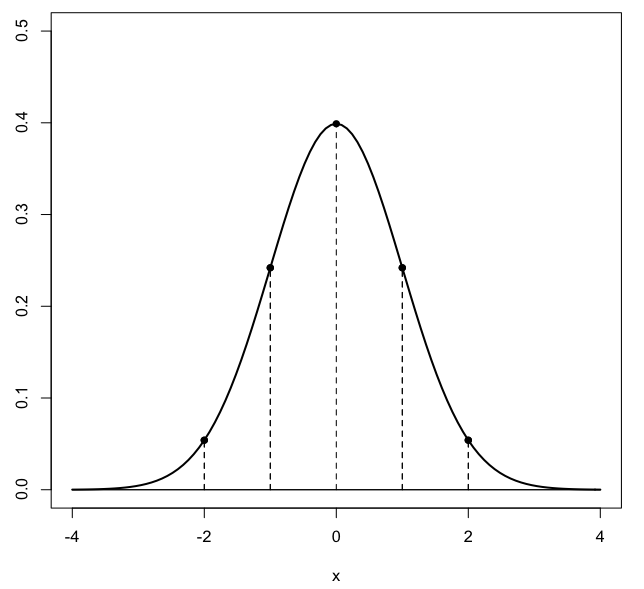
\includegraphics [scale=0.4] {gauss3.png} \end{center}

\title{More about generators}
\date{}

\begin{document}
\maketitle

\Large
To summarize where we are, we're working with a specific Galois field that is useful in cryptography, $GF(2^8)$.  

This field contains the multiplicative identity $1 =$ \textbf{0x01} (but not \textbf{0x00}), as well as 254 additional elements, namely the integers in $[2,255]$ or hex values in \textbf{0x02-0xff}.

Addition is defined simply as $\oplus$ (XOR).  Each element is its own additive inverse (since $a \oplus a = 0$ for every $a$), so subtraction is the same as addition.

$GF(2^8)$ is a finite field.  To achieve this, if addition would result in a value larger than $255$ = \textbf{0xff}, we take the modulus with a special value, called $m(x)$.  Taking the modulus means keeping the remainder from division.

For reasons that we need to explore, $m(x)$ is binary \textbf{1 0001 1011}.  For any number, no matter how large, we could take the modulus by repeated subtraction of $m(x)$.

To do this in binary:  $\oplus$ the value with \textbf{1 0001 1011}.

In decimal, we just say that if the result is $> 255$, first take the remainder from division by $256$, and then $\oplus$ with the number given by the low bits of $m(x)$, namely \textbf{1 1011} = decimal $27$.

It is worth pointing out that we can do everything in decimal and then convert to hex for convenient output if that is desired.  It is actually easier to code in decimal.

\subsection*{multiplication}

To multiply by $2$, multiply by 2 (!), but then take the remainder from division by $256$ and $\oplus \ 27$.  If the multiplicand is $< 128$ only the multiplication is necessary.  In binary, multiply and then do $\oplus$ \textbf{1 0001 1011}.  

To multiply by a power of 2 such as $2^n$, multiply by 2, $n$ times.

To multiply by any other number, decompose the number into its constituent powers of two, do those multiplications, and then add the results by the $\oplus$ operation.

If there is a possibility of generating a number larger than $2^9 - 1$, then we might have to do repeated $\oplus$ (division) or some other method to reduce the result.  It is possible to wait until the very end to do the $\oplus$, but it's often advantageous to do mod as we go.

\subsection*{generators}
In implementing AES, my first approach was to copy tables that list the results of multiplying all numbers in $[0,255]$ by the numbers $2, 3, 9, 11, 13, 14$.

My second approach was to use the algorithm described above to generate such tables.

Then I discovered some pages about generators, which leads to a third approach.

It turns out that fields such as the one we're working with have the property that particular numbers may be generators (also called primitive elements) for the entire field, in the following sense:  all elements of the field can be written as $g^i$ for some positive integer $i$ and generator $g$.  

In particular, \textbf{0x03} is a generator for $GF(2^8)$.  if we implement multiplication by $3$ as described above (that is, with $\oplus \ 27$), and generate the powers from $3^2$ to $3^{255}$, we will generate all the values $[1,255]$, all the values in the field, as a result.  They will be generated in some order (obviously not the usual order) as a list of 255 values.

What is great about this is we can implement multiplication using this table of exponents of $g$, which can simply be added.  It is just the idea of logarithms in a new context.  

We start by reversing the list of exponents to make a list of logarithms. For each index $i$ into the exponents list, find the value of that power, call it $j$ (equal to $g^i$), then find the index $j$ in the logarithms list and write the value $i$ there.  The first list maps the values $[1,255]$ uniquely to the same set of values --- the relationship is bijective, or one-to-one.

To multiply $a \times b$, look up each logarithm in the second table, add the two together, and look up the anti-logarithm in the first table.  That is your result.  The beauty is there is no approximation and no need for interpolation.  The result is exact.  (If you remember interpolating log tables, you are not alone.  There is none of that).

There are other generators for $GF(2^8)$, but \textbf{0x03} is the smallest.  I am curious about what other numbers might be generators for the field.

\subsection*{coding the matrix}

\begin{verbatim}
def normalized(n):
    #  mod 100011011 but only if
    # n >= 0b100000000
    if n < 256:
        return n
    return (n % 256) ^ 27

def times2(n):
    r = n << 1
    return normalized(r)

L = [times2(n) for n in range(256)]
\end{verbatim}
With appropriate formatting code (nothing special), we can print the result as hex or ints:
\begin{verbatim}
00 02 04 06 08 0a 0c 0e 10 12 14 16 18 1a 1c 1e
20 22 24 26 28 2a 2c 2e 30 32 34 36 38 3a 3c 3e
..
db d9 df dd d3 d1 d7 d5 cb c9 cf cd c3 c1 c7 c5
fb f9 ff fd f3 f1 f7 f5 eb e9 ef ed e3 e1 e7 e5 
\end{verbatim}
You can see visually that something different is going on in the lower half of the table.  

I prefer to keep values as integers, save the hex formatting for display and input.  With code to multiply by $3$ and generate its powers, we are ready for the main event.
\begin{verbatim}
def times3(n):
    r = (n << 1) ^ n
    return normalized(r) 

def field_generator():
    n = 1
    while True:
        yield n
        n = times3(n)

g = field_generator()
expL = [g.next() for i in range(256)]
\end{verbatim}

Here is the table of

\textbf{powers}:
\begin{verbatim}
  1   3   5  15  17  51  85 255  26  46 114 150 161 248  19  53
 95 225  56  72 216 115 149 164 247   2   6  10  30  34 102 170
..
 18  54  90 238  41 123 141 140 143 138 133 148 167 242  13  23
 57  75 221 124 132 151 162 253  28  36 108 180 199  82 246   1
\end{verbatim}

I really prefer it as ints, but if you want to compare with the one we found on the web before:
\begin{verbatim}
01 03 05 0f 11 33 55 ff 1a 2e 72 96 a1 f8 13 35
5f e1 38 48 d8 73 95 a4 f7 02 06 0a 1e 22 66 aa
..
12 36 5a ee 29 7b 8d 8c 8f 8a 85 94 a7 f2 0d 17
39 4b dd 7c 84 97 a2 fd 1c 24 6c b4 c7 52 f6 01
\end{verbatim}

To construct a table of logarithms, 
\begin{verbatim}
def makeLogs(expL):
    logL = [None] * 256
    for i in range(256):
        v = expL[i]
        logL[v] = i
    logL[1] = 0
    return logL
\end{verbatim}

Here is the table of

\textbf{logarithms}:
\begin{verbatim}
      0  25   1  50   2  26 198  75 199  27 104  51 238 223   3
100   4 224  14  52 141 129 239  76 113   8 200 248 105  28 193
..
 68  17 146 217  35  32  46 137 180 124 184  38 119 153 227 165
103  74 237 222 197  49 254  24  13  99 140 128 192 247 112   7
\end{verbatim}

Write the int versions of both tables to disk and we are ready to move on.   To test the tables, I started by proofing them against the versions in the source.

I also compared the results of doing multiplication in the standard way for all possible pairs of values.  (I confess that at first I used 100,000 random pairs).  The standard method uses a group of functions like this one for times 4:

\begin{verbatim}
def x4(n):
    if (4,n) in D:  return D[(4,n)]
    ret = normalized(x2(x2(n)))
    D[(4,n)] = ret
    return ret
\end{verbatim}

We use a dictionary to cache the results of computations we've done before.  The call to \textbf{x4} occurs 32640 times.

One tricky thing about the log table is the absence of a value for log(0) since, as usual, the number 0 cannot be generated as a power of $g^i$.  I use the Python value \textbf{None} as a placeholder.

The log table can also be used to easily construct a table of multiplicative inverses.  Any two numbers whose values in the logarithms table add up to \textbf{0xff}, with an anti-logarithm of $1$, have this relationship.  They are multiplicative inverses because when multiplied together they give 1 as the result.

Here is the complete table (in hex) of \textbf{multiplicative inverses}:
\begin{verbatim}
   01 8d f6 cb 52 7b d1 e8 4f 29 c0 b0 e1 e5 c7
74 b4 aa 4b 99 2b 60 5f 58 3f fd cc ff 40 ee b2
3a 6e 5a f1 55 4d a8 c9 c1 0a 98 15 30 44 a2 c2
2c 45 92 6c f3 39 66 42 f2 35 20 6f 77 bb 59 19
1d fe 37 67 2d 31 f5 69 a7 64 ab 13 54 25 e9 09
ed 5c 05 ca 4c 24 87 bf 18 3e 22 f0 51 ec 61 17
16 5e af d3 49 a6 36 43 f4 47 91 df 33 93 21 3b
79 b7 97 85 10 b5 ba 3c b6 70 d0 06 a1 fa 81 82
83 7e 7f 80 96 73 be 56 9b 9e 95 d9 f7 02 b9 a4
de 6a 32 6d d8 8a 84 72 2a 14 9f 88 f9 dc 89 9a
fb 7c 2e c3 8f b8 65 48 26 c8 12 4a ce e7 d2 62
0c e0 1f ef 11 75 78 71 a5 8e 76 3d bd bc 86 57
0b 28 2f a3 da d4 e4 0f a9 27 53 04 1b fc ac e6
7a 07 ae 63 c5 db e2 ea 94 8b c4 d5 9d f8 90 6b
b1 0d d6 eb c6 0e cf ad 08 4e d7 e3 5d 50 1e b3
5b 23 38 34 68 46 03 8c dd 9c 7d a0 cd 1a 41 1c
\end{verbatim}

Note the tricky feature that the exponents and logarithms repeat after 255 values, not 256.  That's because 0 is special in multiplication (even more special than 1).

By playing around I found that \textbf{0x05} is also a generator for the field.  Multiplying by \textbf{0x05} is like multiplying by \textbf{0x03} and then left-shifting by one.  The result can be seen by comparing the first lines of the two tables of exponents:

\begin{verbatim}
01 03 05 0f 11 33 55 ff 1a 2e 72 96 a1 f8 13 35

01 05 11 55 1a 72 a1 13 5f 38 d8 95 f7 06 1e 66
\end{verbatim}

We pick out every second value for the \textbf{0x05}.  The missing values appear starting in the middle of the table.

\begin{verbatim}
03 0f 33 ff 2e 96 f8 35 e1 48 73 a4 02 0a 22 aa
\end{verbatim}

Of course, the logarithms are different with the new generator, but the results of multiplication should be (and appear to be) the same.  For example \textbf{0x53 $\times$ 0xca = 0xff = 0x01}, as before.

I tried some other values for the generator.  I simply tested how many rounds of multiplication it takes before we generate \textbf{0x01} as the power of $g$.  These worked:  3, 5, 6, 9, 11.  These failed after emitting the indicated number of values:  2(51), 4(51), 7(85), 8(17), 10(85).  I didn't test the tables from 5, 6, 9, and 11 extensively but I would be really surprised if they do not work.





\end{document}